 \thispagestyle{cackithitoannone}
\pagestyle{cackithitoan}
\everymath{\color{cackithi}}
\graphicspath{{../cackithi/pic/}}
\blfootnote{{\color[named]{cackithi}$^1$Trường THPT chuyên Khoa học Tự nhiên, Đại học KHTN, Đại học Quốc Gia Hà Nội.}}
\begingroup
\AddToShipoutPicture*{\put(0,616){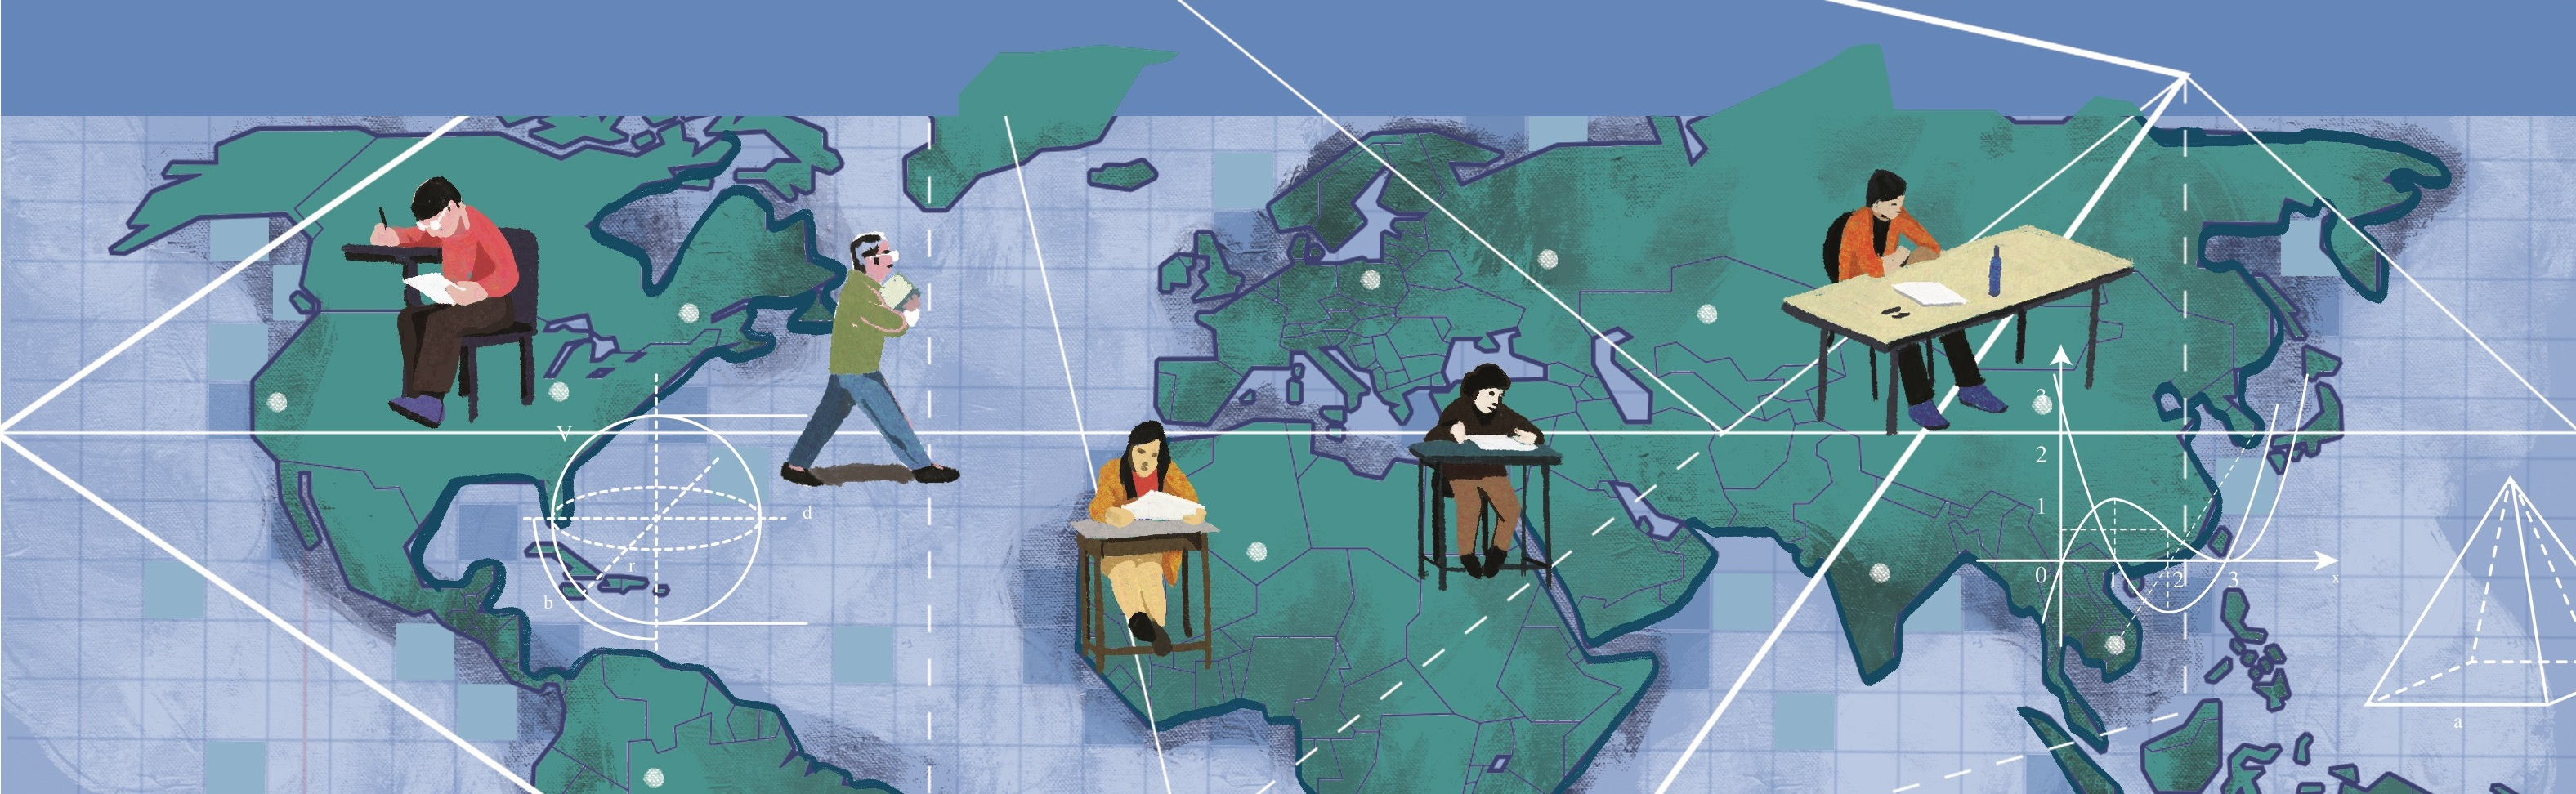
\includegraphics[width=19.3cm]{../bannercackithi}}}
\AddToShipoutPicture*{\put(80,520){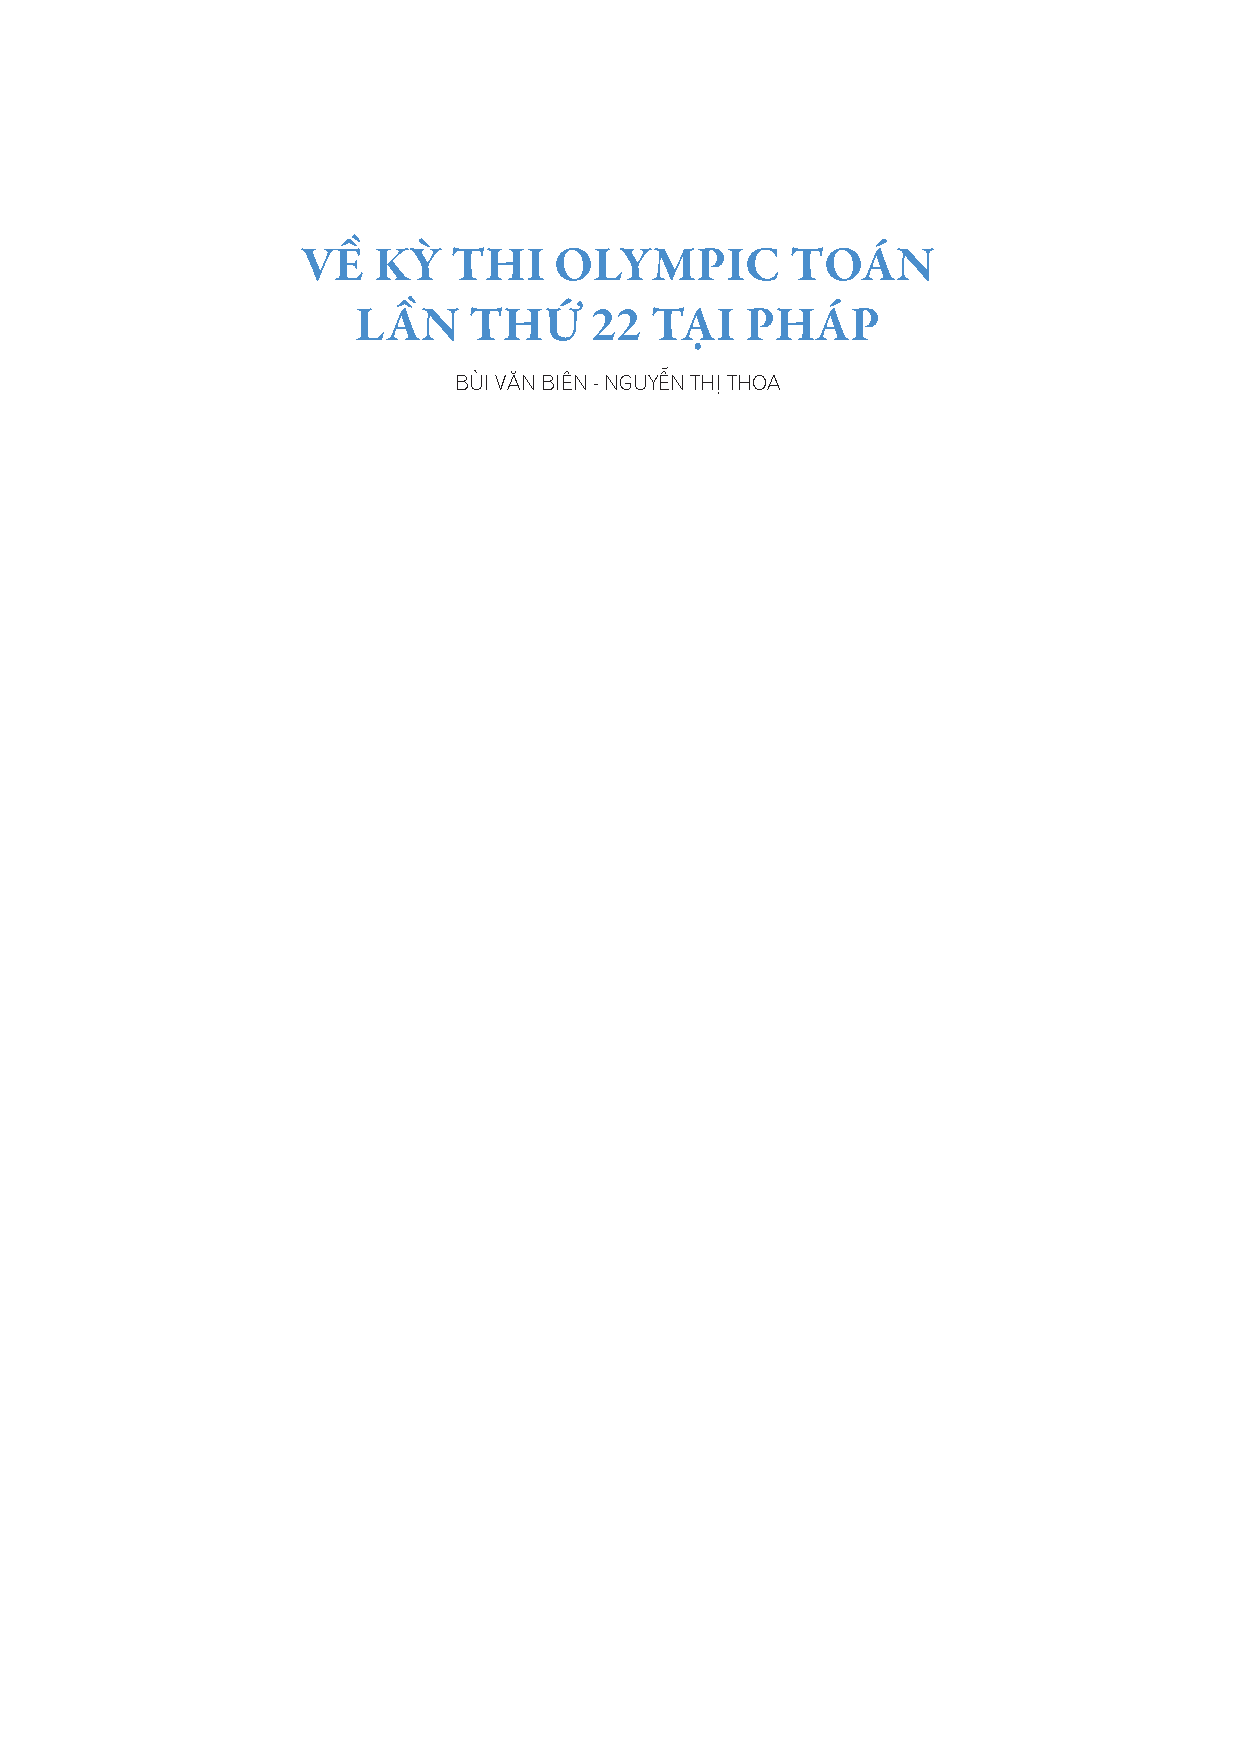
\includegraphics[scale=1]{../tieude.pdf}}} 
\centering
\endgroup
\vspace*{195pt}

	\textbf{\color{cackithi}\emph{LTS.}} Trong Kỳ thi Olympic Toán học sinh viên và học sinh năm $2022$, diễn ra vào các ngày $23$ và $24$ tháng $4$ vừa qua, đề thi dành cho học sinh phổ thông gồm hai bài thi về các chủ đề hình học và số học. Tạp chí Pi giới thiệu với bạn đọc một bài viết thảo luận về các bài toán trong bài thi về chủ đề hình học tại kỳ thi này.   
\begin{multicols}{2}
	$\pmb{1.}$ \textbf{\color{cackithi}Mở đầu}
	\vskip 0.1cm
	Fermat ($1607-1665$) nổi tiếng nhất với công trình nghiên cứu lý thuyết số. Hầu hết chúng ta sẽ biết đến tên của ông nhờ định lý cuối cùng nổi tiếng của ông mà chứng minh của nó thách thức các nhà toán học trong hơn $350$ năm. Cuối cùng, mãi cho đến năm $1995$, chứng minh hoàn chỉnh của nó mới được nhà toán học Anh Andrew Wiles tìm ra. Cuộc sống của Fermat khá bí ẩn. Ông được đào tạo về luật tại Đại học Toulouse của Pháp. Không ai biết ông đã học toán ở đâu. Sau đó, ông chuyển sang Đại học Bordeaux, nơi ông đã làm việc như một luật sư. Ở đó ông bắt đầu tương tác với những bộ óc hàng đầu khi đó như Pascal, Descartes, Galileo, Newton và Torricelli. Fermat thường đặt ra vấn đề và thảo luận với những nhà toán học trên để tìm lời giải. Fermat thường được coi là nhà toán học nghiệp dư vĩ đại cuối cùng. Trong khi nhiều người đã tìm hiểu sâu về cuộc đời của Fermat và định lý cuối cùng nổi tiếng của ông, chúng ta sẽ xem xét kỹ hơn một trong những khám phá ít được biết đến của ông, điểm Fermat. Trong một bức thư riêng gửi Evangelista Torricelli khoảng năm $1640$, Fermat đã đề ra vấn đề sau: 
	\vskip 0.1cm
	{\bf\color{cackithi}Bài toán Fermat.} Cho một tam giác bất kỳ. Hãy tìm một điểm sao cho tổng khoảng cách từ điểm đó tới ba đỉnh của tam giác là nhỏ nhất? 
	\vskip 0.1cm
	Ít lâu sau đó, Torricelli đã đưa ra lời giải mang tính hình học cho bài toán này (xem [$1$]). Vì thế nên điểm thỏa mãn tính chất cực trị này trong tam giác thường mang tên hai ông, \emph{điểm Fermat--Torricelli}.
	\vskip 0.1cm
	Evangelista Torricelli ($1608-1647$) sinh ra ở Faenza, Romagna, Ý, vào năm $1608$. Ông là con cả trong một gia đình có ba người con trai. Khi cha mẹ ông nhận ra tài năng giải quyết vấn đề của ông, họ đã gửi ông cho người bác của ông để ông có một nền ``giáo dục tốt". Bác của Torricelli là một mục sư người Camalonese, Ý. Ông gửi Torricelli đến một trường dòng để ông học toán và triết học. Sau khi tốt nghiệp, Torricelli mong muốn được học cao hơn nữa. Torricelli được giảng dạy về toán học, cơ học, thủy lực học và thiên văn học cổ điển. Ông say mê các tác phẩm của Galileo và sớm bắt đầu trao đổi thư từ với nhà thiên văn học nổi tiếng này. Torricelli trở nên rất quan tâm đến thiên văn học nhưng vào năm $1633$, ông chuyển sang nghiên cứu toán học. Torricelli cuối cùng chuyển đến Arcetri để sống và làm trợ lý cho Galileo. Tuy nhiên, ông chỉ ở đó trong một thời gian rất ngắn ngủi. Về sau, khi Galileo bị xét xử và truy tố vì những công trình thiên văn nổi tiếng của mình về việc Trái Đất quay quanh Mặt Trời thì Torricelli tiếp tục kế vị Galileo nghiên cứu toán và thiên \linebreak văn (xem [$1$]).
	\vskip 0.1cm
	Mặc dù ít được biết tới (so với định lý lớn Fermat), bài toán về điểm Fermat--Torricelli đóng một vai trò vô cùng quan trọng trong hình học của tam giác.
	\vskip 0.1cm
	Nếu các góc của tam giác $ABC$ đều nhỏ hơn $120^\circ$ thì điểm Fermat--Torricelli $T$ nằm trong tam giác $ABC$ và nhìn các cạnh $BC$, $CA$, $AB$ dưới góc $120^\circ$. Để dựng được điểm $T$ của tam giác $ABC$ như vậy, ta có thể dựng ra ngoài tam giác $ABC$ các tam giác đều $BCD$, $CAE$, $ABF$ khi đó đường tròn ngoại tiếp các tam giác đều này sẽ đi qua $T$.
	\begin{figure}[H]
		\vspace*{-5pt}
		\centering
		\captionsetup{labelformat= empty, justification=centering}
		\includegraphics[width= 0.9\linewidth]{figure8053}
		\caption{\small\textit{\color{cackithi}Hình $1.$ Các đường tròn ngoại tiếp tam giác đều đi qua điểm Fermat--Torricelli.}}
		\vspace*{-5pt}
	\end{figure}
	$\pmb{2.}$ \textbf{\color{cackithi}Một số mở rộng đối với tam giác}
	\vskip 0.1cm
	Trong cách dựng điểm Fermat--Torricelli $T$ của tam giác $ABC$ như trên, ta có thể dễ chỉ ra các đường thẳng $AD$, $BE$, $CF$ cùng đi qua $T$. Nếu một cách hình thức, khi $ABC$ là một tam giác bất kỳ, dựng ra ngoài tam giác $ABC$ các tam giác đều $BCD$, $CAE$, $ABF$ thì các đường thẳng $AD$, $BE$, $CF$ vẫn đồng quy; ta gọi điểm đồng quy này là \emph{điểm Fermat--Torricelli thứ nhất của tam giác}, ký hiệu là $F^+$. Để có \emph{điểm Fermat--Torricelli thứ hai của tam giác, ký hiệu là $F^-$}, ta dựng vào trong tam giác $ABC$ các tam giác đều $BCD$, $CAE$, $ABF$, khi đó các đường thẳng $AD$, $BE$, $CF$ đồng quy tại $F^-$.
	\begin{figure}[H]
		\vspace*{-5pt}
		\centering
		\captionsetup{labelformat= empty, justification=centering}
		\includegraphics[width= 0.9\linewidth]{figure8054}
		\caption{\small\textit{\color{cackithi}Hình $2.$ Các đường thẳng $AD$, $BE$, $CF$ đồng quy tại điểm Fermat--Torricelli $T$.}}
		\vspace*{-10pt}
	\end{figure}
	Như vậy nếu mở rộng hơn theo cách dựng các tam giác đều ra ngoài hoặc vào trong, mỗi tam giác sẽ có hai điểm Fermat. Tuy nhiên, điểm Fermat mang tính chất cực trị ứng với các tam giác đều dựng ra ngoài tam giác.
	\vskip 0.1cm
	Một trong những kết quả đẹp và kinh điển của hình học tam giác liên quan tới cả hai điểm Fermat là kết quả sau đây, được Giáo sư Toán học người Canada June Lester công bố trong [$2$].
	\vskip 0.1cm
	{\bf\color{cackithi}Định lý Lester.} Trong một tam giác, hai điểm Fermat, tâm đường tròn ngoại tiếp và tâm đường tròn chín điểm cùng nằm trên một đường tròn.
	\vskip 0.1cm
	Trong đó, đường tròn chín điểm, hay còn gọi là đường tròn Euler của tam giác, là đường tròn đi qua trung điểm của ba cạnh, chân của ba đường cao và trung điểm của ba đoạn thẳng nối trực tâm và các đỉnh tam giác đó. Một lời giải sơ cấp cho định lý Lester có thể tìm thấy trong [$4$].
	\begin{figure}[H]
		\vspace*{-5pt}
		\centering
		\captionsetup{labelformat= empty, justification=centering}
		\includegraphics[width= 0.85\linewidth]{figure8055}
		\caption{\small\textit{\color{cackithi}Hình $3$. Minh họa cho định lý Lester}}
		\vspace*{-10pt}
	\end{figure}
	Điểm Fermat thu được từ việc dựng ra ngoài tam giác $ABC$ ba tam giác đều liên quan mật thiết tới định lý Napoleon sau:
	\vskip 0.1cm
	\noindent{\bf\color{cackithi} Định lý Napoleon.} Tâm của ba tam giác đều dựng ra ngoài một tam giác bất kỳ tạo thành một tam giác đều. Tam giác đều này được gọi là tam giác Napoleon của tam giác đã cho.
	\vskip 0.1cm
	Napoleon ($1769-1821$) là hoàng đế nổi tiếng của nước Pháp. Theo một giai thoại thì ông tìm ra kết quả này trên đường đi chinh chiến. Tuy nhiên, bạn đọc có thể tham khảo một tài liệu nghiên cứu sâu hơn về lịch sử toán học [$3$] để biết rõ hơn về điều này.
	\vskip 0.1cm
	Cũng giống như điểm Fermat, khi ta dựng vào trong tam giác ban đầu ba tam giác đều thì tâm của ba tam giác này cũng tạo thành một tam giác đều, vậy ta có thể coi đây là tam giác Napoleon thứ hai; còn tam giác trên là tam giác Napoleon thứ nhất. Các đường thẳng nối các đỉnh của tam giác $ABC$ và hai tam giác Napoleon của nó cũng 
	đồng quy.
	\vskip 0.1cm
	Mở rộng hơn kết quả đồng quy của hai điểm Fermat và hai tam giác Napoleon, ta có định lý sau đây.
	\vskip 0.1cm
	{\bf\color{cackithi} Định lý Kiepert.} Cho tam giác $ABC$. Dựng ra ngoài tam giác $ABC$ ba tam giác đồng dạng $DBC$, $ECA$, $FAB$ tương ứng cân tại $D$, $E$, $F$. Khi đó $AD$, $BE$, $CF$ đồng quy.
	\begin{figure}[H]
		\vspace*{-5pt}
		\centering
		\captionsetup{labelformat= empty, justification=centering}
		\includegraphics[width= 0.75\linewidth]{figure8056}
		\caption{\small\textit{\color{cackithi}Hình $4$. Minh họa cho định lý Kiepert.}}
		\vspace*{-10pt}
	\end{figure}
	Ludwig Kiepert ($1846-1934$) là một nhà toán học người Đức, là giáo sư toán học tại Hannover Technische Hochschule, Đức. Ông có các nghiên cứu về hình học và giải tích. Trong đó định lý trên của Kiepert dẫn đến những nghiên cứu sâu hơn trong hình học tam giác.
	\vskip 0.1cm
	Vì tính chất quan trọng của định lý Kiepert, chúng tôi xin giới thiệu một chứng minh dựa trên định lý Ceva về ba đường đồng quy.
	\begin{figure}[H]
		\vspace*{-5pt}
		\centering
		\captionsetup{labelformat= empty, justification=centering}
		\includegraphics[width= 0.75\linewidth]{figure8056a}
		\caption{\small\textit{\color{cackithi}Hình $5$. Minh họa cho chứng minh của định lý Kiepert.}}
		\vspace*{-10pt}
	\end{figure}
	\textit{Chứng minh định lý Kiepert.} Do các tam giác $DBC$, $ECA$, $FAB$ cân tại $D$, $E$, $F$ và đồng dạng. Ta đặt
		\begin{align*}
			\angle DBC&=\angle DCB=\angle ECA=\angle EAC\\
			&=\angle FAB=\angle FBA=\theta.
		\end{align*}
		Đặt $BC=a$, $CA=b$, $AB=c$. Gọi giao điểm của $AD$, $BE$, $CF$ với các cạnh $BC$, $CA$, $AB$ theo thứ tự là $X$, $Y$, $Z$. Ký hiệu $[UVW]$ là diện tích tam giác $UVW$, ta có
		\begin{align*}
			\frac{XB}{XC}&=\frac{[ABD]}{[ACD]}=\frac{\frac{1}{2}BA\cdot BD\sin\angle ABD}{\frac{1}{2}CA\cdot CD\sin\angle ACD}\\
			&=\frac{c\sin(\theta+\angle B)}{b\sin(\theta+\angle C)}. \tag{$1$}
		\end{align*}
		Chứng minh tương tự, ta có
		\begin{align*}\frac{YC}{YA}=\frac{a\sin(\theta+\angle C)}{c\sin(\theta+\angle A)}\tag{$2$}
		\end{align*}
		và
		\begin{align*}\label{eq3}\frac{ZA}{ZB}=\frac{b\sin(\theta+\angle A)}{a\sin(\theta+\angle B)}.\tag{$3$}
		\end{align*}
		Từ ($1$), ($2$), ($3$), ta suy ra
		\begin{align*}
			&\frac{XB}{XC}\cdot\frac{YC}{YA}\cdot\frac{ZA}{ZB}\\
			=&\frac{c\sin(\!\theta\!+\!\angle B)}{b\sin(\!\theta\!+\!\angle C)}\!\cdot\!\frac{a\sin(\!\theta\!+\!\angle C)}{b\sin(\!\theta\!+\!\angle A)}\!\cdot\!\frac{b\sin(\!\theta\!+\!\angle A)}{a\sin(\!\theta\!+\!\angle B)}\\
			=&1.
		\end{align*}
		Vậy theo định lý Ceva đảo thì $AX$, $BY$, $CZ$ đồng quy hay $AD$, $BE$, $CF$ đồng quy. Ta hoàn tất chứng minh.
	\vskip 0.1cm
	$\pmb{3.}$ \textbf{\color{cackithi}Lời giải và các mở rộng của bài toán Fermat}
	\vskip 0.1cm
	Trong suốt quá trình lịch sử từ khi bài toán được đặt ra thì bài toán Fermat được nhiều người quan tâm và giải quyết cũng như mở rộng, phát triển, tổng quát nó. Kể từ lời giải sớm nhất của Torricelli mang tính hình học (xem [$6$]), thì đã có một lượng lớn các lời giải khác nhau ra đời với nhiều phương pháp tiếp cận như dùng phép quay các tam giác đều, dùng tọa độ Descartes, dùng giải tích, dùng tích vô hướng  v.v. (xem [$7$]).
	\vskip 0.1cm
	Bài toán Fermat cũng có nhiều mở rộng tổng quát như chúng ta thay tam giác thành đa giác, thay vì tìm vị trí một điểm mà tổng khoảng cách là nhỏ nhất thì ta có thể tìm vị trí nhiều điểm để tổng khoảng cách bé nhất. Cách mở rộng này là của Jakob Steiner và đưa tới những nghiên cứu sâu hơn trong lý thuyết đồ thị, xem [$8$]. 
	
	Mặt khác, cũng có nhiều mở rộng bài toán Fermat trên tam giác như thêm trọng số (cả trọng số dương và trọng số âm) [$9, 11$], mở rộng với số mũ [$10$], mở rộng trên đa tạp và không gian nhiều chiều [$12$].
	\vskip 0.1cm
	$\pmb{4.}$ \textbf{\color{cackithi}Trong hình học của tam giác và trong các kỳ thi toán}
	\vskip 0.1cm
	Đối với hình học của tam giác, hai điểm Fermat đóng một vài trò quan trọng [$13,14$]. Như đã nói ở trên, định lý Lester, liên quan tới cả hai điểm Fermat, cũng có ý nghĩa lớn trong hình học của tam giác. Vì điều đặc biệt đó mà ngoài ý nghĩa của bài toán cực trị (bài toán Fermat) thì điểm Fermat cũng được khai thác dưới góc độ hình học của tam giác với nhiều khai thác và phát triển, rất nhiều kết quả được chỉ ra và chứng minh trong [$15,16,17,18,19$].
	\vskip 0.1cm
	Gần đây, trong kỳ thi Olympic Toán học sinh viên và học sinh năm $2022$, do hội toán học Việt Nam (VMS) tổ chức, đề thi dành cho học sinh về chủ đề hình học cũng khai thác chuỗi gồm $8$ bài toán liên quan tới điểm Fermat--Torricelli của tam giác. Chúng tôi xin giới thiệu với bạn đọc các bài toán của kỳ thi kể trên.
	\vskip 0.1cm
	\textbf{\color{cackithi}Bài toán $\pmb{1}$} (điểm Fermat--Torricelli)\textbf{\color{cackithi}.} Chứng minh rằng tồn tại duy nhất một điểm $T$ nằm trong tam giác $ABC$ (với các góc nhỏ hơn $120^\circ$) sao cho $\angle BTC = \angle CTA = \angle ATB=120^{\circ}$. Điểm $T$ xác định như vậy được gọi là điểm Fermat--Torricelli của tam giác $ABC$. 
	\vskip 0.1cm
	\textit{Chứng minh.} Dựng $2$ cung chứa góc  $120^\circ$ trên các cạnh $BC$, $CA$  nằm trong tam giác. Gọi $T $ là giao điểm thứ $2$ (khác $C$) của $2$ cung trên. Do tính chất của tam giác $ABC$, dễ thấy $T$ tồn tại và duy nhất. Mặt khác, từ cách dựng $T$, ta có  $\angle BTC = \angle CTA = \angle ATB=120^{\circ}$.
	\vskip 0.1cm
	{\bf\color{cackithi} Bình luận.} Bài toán nêu yêu cầu rõ ràng là chứng minh tồn tại và duy nhất. Vậy thì cách dựng cung chứa góc cắt nhau đã chỉ ra là luôn tồn tại (vì cung chứa góc luôn tồn tại, đồng thời chúng luôn cắt nhau). Còn tính duy nhất vì giao điểm thứ hai thì hiển nhiên là duy nhất.
	\vskip 0.1cm
	\textbf{\color{cackithi}Bài toán $\pmb{2}$} (Cách dựng khác cho điểm Fermat--Torricelli)\textbf{\color{cackithi}.} Dựng ra ngoài tam giác $ABC$ ba tam giác đều $BCD$, $CAE$, $ABF$. Chứng minh rằng $AD$, $BE$, $CF$ đồng quy tại~$T$.
	\begin{figure}[H]
		\vspace*{-5pt}
		\centering
		\captionsetup{labelformat= empty, justification=centering}
		\includegraphics[width= 0.75\linewidth]{figure7793}
		\vspace*{-15pt}
	\end{figure}
	\textit{Chứng minh.} Theo định nghĩa $\angle BTC=\angle CTA=\angle ATC=120^\circ$ nên các tứ giác $ATCE$, $BTCD$, $BTAF$ nội tiếp. Từ đó $\angle ATF=\angle ABF=60^\circ$, $\angle FTB=\angle FAB=60^\circ$, và $\angle BTD=\angle BCD=60^\circ$. Vậy $\angle ATD=180^\circ$ hay $A$, $T$, $D$ thẳng hàng. Chứng minh tương tự, $BE$, $CF$ đi qua $T$.
	\vskip 0.1cm
	{\bf\color{cackithi} Bình luận.} Bài toán này có thể coi là ta chứng minh lại định lý Kiepert, khi dựng ra ngoài các tam giác đều $BCD$, $CAE$, $ABF$ thì các đường thẳng $AD$, $BE$, $CF$ đồng quy. Đây là cách chứng minh thuần túy hình học, không dùng định lý Ceva.
	\vskip 0.1cm
	\textbf{\color{cackithi}Bài toán $\pmb{3}$} (Bài toán Fermat)\textbf{\color{cackithi}.} Xét một điểm $P$ nằm trong mặt phẳng chứa tam giác $ABC$ (với các góc nhỏ hơn $120^\circ$). Gọi $T$ là điểm Fermat--Torricelli của tam giác $ABC$. Chứng minh rằng
	\vskip 0.1cm
	$a)$  \begin{align*}
		\frac{\overrightarrow{TA}}{TA}+\frac{\overrightarrow{TB}}{TB}+\frac{\overrightarrow{TC}}{TC}=\overrightarrow{0}.
	\end{align*}
	$b)$\begin{align*}
		PA\!+\! PB\!+\!PC \!\ge\! \frac{\overrightarrow{PA}\!\cdot\!\overrightarrow{TA}}{TA}\!+\!\frac{\overrightarrow{PB}\!\cdot\! \overrightarrow{TB}}{TB}\!+\!\frac{\overrightarrow{PC}\!\cdot\!\overrightarrow{TC}}{TC}.
	\end{align*}
	$c)$
	\begin{align*}
		PA+PB+PC\ge TA+TB+TC
	\end{align*}
	và đẳng thức xảy ra khi và chỉ khi $P$ trùng với $T$. 
	\vskip 0.1cm
	\textit{Lời giải.} $a)$ Do các vector $\frac{\overrightarrow{TA}}{TA}$, $\frac{\overrightarrow{TB}}{TB}$, $\frac{\overrightarrow{TC}}{TC}$ có độ dài bằng nhau (bằng $1$) và đặt lệch nhau các góc $120^\circ$ nên
	\begin{align*}
		\frac{\overrightarrow{TA}}{TA}+\frac{\overrightarrow{TB}}{TB}+\frac{\overrightarrow{TC}}{TC}=\overrightarrow{0}.
	\end{align*}
	$b)$ $c)$ Sử dụng bất đẳng thức với tích vô hướng và các tính chất của tích vô hướng, với mọi $P$, ta có
		\begin{align*}
			&PA+PB+PC\\[-0.2ex]
			=\,&\frac{PA\cdot TA}{TA}+\frac{PB\cdot TB}{TB}+\frac{PC\cdot TC}{TC}\\[-0.2ex]
			\ge\,& \frac{\overrightarrow{PA}\cdot\overrightarrow{TA}}{TA}+\frac{\overrightarrow{PB}\cdot \overrightarrow{TB}}{TB}+\frac{\overrightarrow{PC}\cdot\overrightarrow{TC}}{TC}\\[-0.2ex]
			=\,&\frac{\left(\overrightarrow{PT}+\overrightarrow{TA}\right)\cdot\overrightarrow{TA}}{TA}+\frac{\left(\overrightarrow{PT}+\overrightarrow{TB}\right)\cdot\overrightarrow{TB}}{TB}\\[-0.2ex]
			&+\frac{\left(\overrightarrow{PT}+\overrightarrow{TC}\right)\cdot\overrightarrow{TC}}{TC}\\[-0.2ex]
			=\,&\overrightarrow{PT}\!\left(\!\frac{\overrightarrow{TA}}{TA}\!+\!\frac{\overrightarrow{TB}}{TB}\!+\!\frac{\overrightarrow{TC}}{TC}\!\right)\!+\!TA\!+\!TB\!+\!TC\\[-0.2ex]
			=\,&TA+TB+TC.
		\end{align*}
		Đẳng thức xảy ra khi và chỉ khi $P$ trùng $T$.
	\vskip 0.1cm
	{\bf\color{cackithi} Bình luận.} Từ tính chất điểm Fermat--Torricelli ta thấy $T$ nhìn các cạnh của tam giác dưới góc $120^\circ$ dẫn tới xuất hiện vector--không $\frac{\overrightarrow{TA}}{TA}+\frac{\overrightarrow{TB}}{TB}+\frac{\overrightarrow{TC}}{TC}=\overrightarrow{0}.$ Để từ đó dùng được tính chất tích vô hướng là một cách giải rất quan trọng cho bài toán Fermat. Nhờ đó ta có thể giải quyết được bài toán Steiner hoặc một số mở rộng của nó với trọng số [$11$] hoặc lên không gian nhiều chiều hơn [$12$].
	\vskip 0.1cm
	\textbf{\color{cackithi}Bài toán $\pmb{4.}$} (Thêm trọng số cho bài toán Fermat)\textbf{\color{cackithi}.} Giả sử tam giác $ABC$ nhọn. Đặt $a=BC$, $b=CA$, $c=AB$.
	\vskip 0.1cm
	$a)$ Ký hiệu $H$ là trực tâm của tam giác $ABC$. Chứng minh rằng 
	\begin{align*}
		a\cdot\frac{\overrightarrow{HA}}{HA}+b\cdot\frac{\overrightarrow{HB}}{HB}+c\cdot\frac{\overrightarrow{HC}}{HC}=\overrightarrow{0}.
	\end{align*}
	$b)$ Xét một điểm $P$ nằm trong mặt phẳng. Chứng minh rằng tổng
	\begin{align*}
		aPA+bPB+cPC
	\end{align*} 
	đạt giá trị nhỏ nhất khi và chỉ khi $P$ trùng với $H$.
	\vskip 0.1cm
	\textit{Chứng minh.}	
		$a)$ Cách $1$: Hệ quả trực tiếp của định lí con nhím.
		\vskip 0.1cm
		Cách $2$: Đặt  $\overrightarrow{u}=a\cdot\dfrac{\overrightarrow{HA}}{HA}+b\cdot\dfrac{\overrightarrow{HB}}{HB}+c\cdot\dfrac{\overrightarrow{HC}}{HC}.$
		Dễ dàng kiểm tra $\overrightarrow{u}\cdot\overrightarrow{AB}=\overrightarrow{u}\cdot\overrightarrow{BC}=0$. Từ đây suy ra $\overrightarrow{u}=\overrightarrow{0}.$
		\vskip 0.1cm
		$b)$ Với mọi $P$ ta có
		\begin{align*}
			&aPA+bPB+cPC\\
			=&\frac{aPA\cdot HA}{HA}+\frac{bPB\cdot HB}{HB}+\frac{cPC\cdot HC}{HC}\\
			\ge&\frac{a\overrightarrow{PA}\cdot \overrightarrow{HA}}{HA}+\frac{b\overrightarrow{PB}\cdot \overrightarrow{HB}}{HB}+\frac{c\overrightarrow{PC}\cdot \overrightarrow{HC}}{HC}\\
			=&\frac{a(\overrightarrow{PH}+\overrightarrow{HA})\cdot \overrightarrow{HA}}{HA}+\frac{b(\overrightarrow{PH}+\overrightarrow{HB})\cdot \overrightarrow{HB}}{HB}\\
			&+\frac{c(\overrightarrow{PH}+\overrightarrow{HC})\cdot \overrightarrow{HC}}{HC}\\
			=&\overrightarrow{PH}\cdot\left(a\cdot\frac{\overrightarrow{HA}}{HA}+b\cdot\frac{\overrightarrow{HB}}{HB}+c\cdot\frac{\overrightarrow{HC}}{HC}\right)\\
			&+aHA+bHB+cHC\\
			=&aHA+bHB+cHC
		\end{align*}
		Dễ thấy dấu bằng xảy ra khi $P=H$ nói cách khác tổng $aPA+bPB+cPC$ đạt giá trị bé nhất khi $P$ là trực tâm tam giác $ABC$.
	\vskip 0.1cm
	{\bf\color{cackithi} Bình luận.} Cách làm trên sử dụng bất đẳng thức với tích vô hướng và dựa vào đẳng thức của vector--không $a\!\cdot\!\frac{\overrightarrow{HA}}{HA}\!+\!b\!\cdot\!\frac{\overrightarrow{HB}}{HB}\!+\!c\!\cdot\!\frac{\overrightarrow{HC}}{HC}\!=\!\overrightarrow{0}$ cũng rất giống cách làm trong bài toán Fermat gốc, bằng cách tương tự, ta có thể tổng quát bài toán này lên với bộ ba số thực dương $x$, $y$, $z$, xem [$11$].
	\vskip 0.1cm
	\textbf{\color{cackithi}Bài toán $\pmb{5}$} (Bài toán Steiner) Cho tứ giác $MNPQ$. Giả sử tồn tại hai điểm $U$ và $V$ nằm trong tứ giác thỏa mãn
	\begin{align*}
		\angle MUN&= \angle MUV= \angle NUV = \angle QVU\\
		&= \angle PVU=\angle PVQ.
	\end{align*}
	Xét hai điểm $X$ và $Y$ trong mặt phẳng. Chứng minh rằng tổng
	\begin{align*}
		XM+XN+XY+YP+YQ
	\end{align*}
	đạt giá trị nhỏ nhất khi và chỉ khi $X=U$ và $Y=V$.
	\begin{figure}[H]
		\vspace*{-5pt}
		\centering
		\captionsetup{labelformat= empty, justification=centering}
		\includegraphics[width= 0.75\linewidth]{figure8058}
		\caption{\small\textit{\color{cackithi}Hình $6$. Minh họa cho lời giải bài toán Steiner.}}
		\vspace*{-10pt}
	\end{figure}
	\textit{Lời giải.} (Xem Hình $6$). Do 
	\begin{align*}
		\angle MUN&=\angle MUV=\angle NUV=\angle QVU\\
		&=\angle PVU=\angle PVQ=120^\circ,
	\end{align*} nên tương tự như trong lời giải bài toán $3$, ta có
		\begin{align*}
			\frac{\overrightarrow{UM}}{UM}+\frac{\overrightarrow{UN}}{UN}+\frac{\overrightarrow{UV}}{UV}=\overrightarrow{0}
		\end{align*}
		và
		\begin{align*}
			\frac{\overrightarrow{VP}}{VP}+\frac{\overrightarrow{VQ}}{VQ}+\frac{\overrightarrow{VU}}{VU}=\overrightarrow{0}.
		\end{align*}
		Từ đó ta có biến đổi bất đẳng thức và tích vô hướng như sau
		\begin{align*}&XM+XN+XY+YP+YQ\\
			=&\frac{XM\cdot UM}{UM}+\frac{XM\cdot UN}{UN}+\frac{XY\cdot UV}{UV}\\
			&+\frac{YP\cdot VP}{VP}+\frac{YQ\cdot VQ}{VQ}\\
			\ge&\frac{\overrightarrow{XM}\cdot \overrightarrow{UM}}{UM}+\frac{\overrightarrow{XN}\cdot \overrightarrow{UN}}{UN}+\frac{\overrightarrow{XY}\cdot \overrightarrow{UV}}{UV}\\
			&+\frac{\overrightarrow{YP}\cdot \overrightarrow{VP}}{VP}+\frac{\overrightarrow{YQ}\cdot\overrightarrow{VQ}}{VQ}\\
			=&\frac{(\overrightarrow{XU}+\overrightarrow{UM})\cdot \overrightarrow{UM}}{UM}+\frac{(\overrightarrow{XU}+\overrightarrow{UN})\cdot \overrightarrow{UN}}{UN}\\
			&+\frac{(\overrightarrow{XU}+\overrightarrow{UV}+\overrightarrow{VY})\cdot \overrightarrow{UV}}{UV}\\
			&+\frac{(\overrightarrow{YV}+\overrightarrow{VP})\cdot \overrightarrow{VP}}{VP}+\frac{(\overrightarrow{YV}+\overrightarrow{VQ})\cdot\overrightarrow{VQ}}{VQ}\\
			=&\overrightarrow{XU}\cdot\left(\frac{\overrightarrow{UM}}{UM}+\frac{\overrightarrow{UN}}{UN}+\frac{\overrightarrow{UV}}{UV}\right)\\
			&+\overrightarrow{YV}\cdot\left(\frac{\overrightarrow{VP}}{VP}+\frac{\overrightarrow{VQ}}{VQ}+\frac{\overrightarrow{VU}}{VU}\right)\\
			&+UM+UN+UV+VQ+VP\\
			=&UM+UN+UV+VQ+VP.
		\end{align*}
		Dấu bằng xảy ra khi $X=U$, $Y=V$. Vậy tổng $XM+XN+XY+YP+YQ$ đạt giá trị bé nhất khi và chỉ khi $X=U$, $Y=V$.
	\vskip 0.1cm
	{\bf\color{cackithi} Bình luận.} Rõ ràng phương pháp vector và tích vô hướng là cách tiếp cận thú vị và ngắn gọn cho bài toán này. Thoạt nhìn bài toán này trông như việc ghép nối hai bài toán Fermat trên tam giác (vì hai tam giác $VMN$ và $UPQ$ lần lượt có hai điểm Fermat là $U$ và $V$). Nhưng sự xuất hiện của đại lượng $UV$ (một lần) trong tổng cần tìm cực trị làm chúng ta không thể dùng hai bài toán Fermat trên tam giác ghép vào được mà bắt buộc phải phân tích vector đưa về các gốc $U$ và $V$ như đã làm. Bài toán cũng có thể giải được bằng cách dựng thêm các tam giác đều ra ngoài tứ giác $MNPQ$.
	\vskip 0.1cm
	\textbf{\color{cackithi}Bài toán $\pmb{6.}$} Gọi $G$ và $T$ lần lượt là trọng tâm và điểm Fermat--Torricellicủa tam giác $ABC$. Chứng minh rằng $G$ cách đều các đường trung trực của các đoạn thẳng $TA$, $TB$, $TC$.
	\begin{figure}[H]
		\vspace*{-5pt}
		\centering
		\captionsetup{labelformat= empty, justification=centering}
		\includegraphics[width= 0.8\linewidth]{figure7794}
		\vspace*{-10pt}
	\end{figure}
	\textit{Chứng minh.} Dựng ra ngoài các tam giác đều $BCD$, $CAE$, $ABF$ có tâm lần lượt là $X$, $Y$, $Z$. Theo bài toán $1$, các tứ giác $ATCE$, $BTCD$, $BTAF$ nội tiếp nên $YZ$, $ZX$, $XY$ lần lượt là trung trực của $TA$, $TB$, $TC$. Dễ thấy do $TA$, $TB$, $TC$ lệch nhau góc $120^\circ$ nên tam giác $XYZ$ đều. Từ đó chỉ cần chứng minh $G$ là trọng tâm tam giác $XYZ$ thì hiển nhiên $G$ cách đều các đường thẳng $YZ$, $ZX$, $XY$ (cũng chính là trung trực $TA$, $TB$, $TC$). Xét 
	\begin{align*}
		\overrightarrow{u}=\overrightarrow{AY}+\overrightarrow{CX}+\overrightarrow{BZ}.
	\end{align*}
	Quay các vector $\overrightarrow{AY}$, $\overrightarrow{CX}$, $\overrightarrow{BZ}$ góc $30^\circ$ cùng chiều kim đồng hồ thì các vector nhận được lần lượt là $\frac{\overrightarrow{AC}}{\sqrt{3}}$, $\frac{\overrightarrow{CB}}{\sqrt{3}}$, $\frac{\overrightarrow{BA}}{\sqrt{3}}$. Hiển nhiên tổng 
	\begin{align*}
		\frac{\overrightarrow{AC}}{\sqrt{3}}+\frac{\overrightarrow{CB}}{\sqrt{3}}+\frac{\overrightarrow{BA}}{\sqrt{3}}=\overrightarrow{0},
	\end{align*}
	ta suy ra $\overrightarrow{u}=\overrightarrow{0}$. Nói cách khác, các tam giác $ABC$ và $XYZ$ có cùng trọng tâm, do đó $G$ là trọng tâm tam giác $XYZ$.
	\vskip 0.1cm
	{\bf\color{cackithi} Bình luận.} Phép quay vector là phương án rất tốt để tiếp cận bài toán này. Nếu không dùng phép quay vector, bạn đọc cũng có thể chứng minh bài toán theo cách vẽ đường phụ, dùng tính chất của trọng tâm tam giác cách mỗi đỉnh bằng $\frac{2}{3}$ độ dài trung tuyến ứng với đỉnh đó.
	\vskip 0.1cm
	\textbf{\color{cackithi}Bài toán $\pmb{7.}$} Gọi $T$ là điểm Fermat--Torricelli của tam giác không cân $ABC$. Gọi $H_a$, $H_b$, $H_c$ tương ứng là trực tâm các tam giác $TBC$, $TCA$, $TAB$.
	\vskip 0.1cm
	$a)$ Chứng minh rằng $T$ là trọng tâm của tam giác $H_aH_bH_c$.
	\vskip 0.1cm
	$b)$ Gọi $D$, $E$, $F$ tương ứng là giao điểm của $H_cH_b$ và cạnh $BC$, $H_cH_a$ và cạnh $CA$, $H_aH_b$ và cạnh $AB$. Chứng minh rằng tam giác $DEF$ đều.
	\vskip 0.1cm
	$c)$ Chứng minh rằng các đường thẳng đi qua $D$, $E$, $F$ và tương ứng vuông góc với $BC$, $CA$, $AB$ đồng quy tại một điểm. Ký hiệu điểm đó là $S$.
	\vskip 0.1cm
	$d)$ Chứng minh rằng $TS$ song song với đường thẳng Euler của tam giác $ABC$.
	\begin{figure}[H]
		\vspace*{-5pt}
		\centering
		\captionsetup{labelformat= empty, justification=centering}
		\includegraphics[width= 0.8\linewidth]{figure7798}
		\vspace*{-5pt}
	\end{figure}
	$a)$ Gọi $M_a$, $M_b$, $M_c$ lần lượt là trung điểm  $BC$, $CA$, $AB$. Gọi $X$, $Y$, $Z$ là tâm ngoại tiếp các tam giác $TBC$, $TCA$, $TAB$. Theo bài toán $6$, hai tam giác $XYZ$ và $ABC$ có cùng trọng tâm. Dễ thấy hai tam giác $ABC$ và $M_aM_bM_c$ có cùng trọng tâm nên tam giác $XYZ$ và $M_aM_bM_c$ có cùng trọng tâm. Vậy
	\begin{align*}
		\overrightarrow{TH_a}\!+\!\overrightarrow{TH_b}\!+\!\overrightarrow{TH_c}
		&=\!2\left(\overrightarrow{XM_a}\!+\!\overrightarrow{YM_b}\!+\!\overrightarrow{ZM_c}\right)\\
		&=\!\overrightarrow{0}.
	\end{align*}
	Hay $T$ là trọng tâm tam giác $H_aH_bH_c$.
	\vskip 0.1cm	
	$b)$, $c)$ Ta có bổ đề sau
	\vskip 0.1cm
	{\bf\color{cackithi} Bổ đề.} Cho tam giác $ABC$ với hai điểm $P$, $Q$ (nằm trong tam giác) đẳng giác đối với tam giác. Gọi $K$, $L$ lần lượt là trực tâm của các tam giác $PCA$, $PAB$. Gọi $D$ là hình chiếu vuông góc của $Q$ lên $BC$. Khi đó ba điểm $K$, $D$, $L$ thẳng hàng.
	\begin{figure}[H]
		\vspace*{-5pt}
		\centering
		\captionsetup{labelformat= empty, justification=centering}
		\includegraphics[width= 0.9\linewidth]{figure3526a}
		\vspace*{-10pt}
	\end{figure}
	{\bf\color{cackithi} Chứng minh.} Gọi giao điểm của $PK,PL$ với $CA,AB$ lần lượt $E,F$. Ta dễ thấy các cặp tam giác đồng dạng $\triangle PBF\sim\triangle QBD$ và $\triangle PCE\sim\triangle QCD$. Ta có biến đổi tỷ số như sau
	\begin{align*}
		\frac{DB}{DC}&=\frac{DB}{DQ}\!\cdot\!\frac{DQ}{DC}\!=\!\frac{BF}{FP}\!\cdot\!\frac{PE}{EC}\!=\!\frac{BF}{EC}\!\cdot\!\frac{PA}{FP}\!\cdot\!\frac{PE}{PA}\\
		&=\frac{BF}{EC}\cdot\frac{BL}{BF}\cdot\frac{CE}{CK}=\frac{BL}{CK}.
	\end{align*} 
	Kết hợp với $BL\parallel CK$, ta suy ra ba điểm $K$, $D$, $L$ thẳng hàng. Kết thúc chứng minh.
	\begin{figure}[H]
%		\vspace*{-5pt}
		\centering
		\captionsetup{labelformat= empty, justification=centering}
		\includegraphics[width= 0.8\linewidth]{figure7799}
		\vspace*{-10pt}
	\end{figure}
	Gọi $S$ là đẳng giác của $T$ trong tam giác $ABC$. Áp dụng bổ đề thì $D$, $E$, $F$ lần lượt là hình chiếu của $S$ trên các cạnh $BC$, $CA$, $AB$. Từ đó, bằng cách cộng góc đơn giản dễ chỉ ra tam giác $DEF$ đều. Hiển nhiên các đường thẳng qua $D$, $E$, $F$ vuông góc $BC$, $CA$, $AB$ đồng quy tại $S$.
	\vskip 0.1cm	
	$d)$ Từ tính chất điểm đẳng giác, dễ thấy $EF$, $FD$, $DE$ lần lượt vuông góc với $TA$, $TB$, $TC$. Gọi $X$, $Y$, $Z$ lần lượt là tâm đường tròn ngoại tiếp các tam giác $TBC$, $TCA$, $TAB$, ta cũng dễ thấy $YZ$, $ZX$, $XY$ lần lượt vuông góc với $TA$, $TB$, $TC$. Từ đó hai tam giác $DEF$ và $XYZ$ có cạnh tương ứng song song nên $DX$, $EY$, $FZ$ đồng quy tại $P$. Xét phép vị tự $\mathcal{H}_P$ tâm $P$ biến tam giác $DEF$ thành $XYZ$. Tâm ngoại tiếp của $DEF$ là trung điểm $J$ của $ST$ biến thành tâm ngoại tiếp tam giác $XYZ$ cũng chính là trọng tâm $G$ của \linebreak$ABC$ (theo Bài $4$). \hfill ($1$)
	\begin{figure}[H]
		\vspace*{-5pt}
		\centering
		\captionsetup{labelformat= empty, justification=centering}
		\includegraphics[width= 0.9\linewidth]{figure7667}
		\vspace*{-10pt}
	\end{figure}
	Các đường thẳng từ $Y$, $Z$ vuông góc với $CA$, $AB$, cắt nhau tại tâm ngoại tiếp $O$ của $ABC$. Các đường vuông góc từ $E$, $F$ với $CA$, $AB$, cắt nhau tại $S$. Dễ thấy phép vị tự $\mathcal{H}_P$ biến $E\mapsto Y$, $F\mapsto Z$ do đó $S\mapsto O$. \hfill($2$)
	\vskip 0.1cm
	Từ ($1$) và ($2$), ta thu được phép vị tự $\mathcal{H}_P$ biến $JS$ (hay chính là $TS$) thành đường thẳng Euler $GO$ của $ABC$, do đó $ST\parallel OG$.
	\vskip 0.1cm
	{\bf\color{cackithi} Bình luận.} Đây là bài toán khá thú vị đề cập đến cả điểm Fermat và điểm liên hợp đẳng giác của điểm Fermat (điểm Isodynamic). Các câu $a)$, $b)$, $c)$ để dùng cho câu $d)$, các ý của bài toán chặt chẽ và liên kết nhau. Như vậy ta có thể tóm gọn ý của bài toán đó là trong một tam giác, đường thẳng nối điểm Fermat và điểm liên hợp đẳng giác của nó song song với đường thẳng Euler của tam giác.
	\vskip 0.1cm
	\textbf{\color{cackithi}Bài toán $\pmb{8.}$} Cho tam giác $ABC$ không cân có điểm Fermat--Torricelli là $T$. Gọi $(N_a)$ là đường tròn ngoại tiếp tam giác $TBC$. Lấy $X$ trên $(N_a)$ sao cho $TX\perp BC$. Gọi giao điểm của đoạn thẳng $BC$ và đường tròn ngoại tiếp tam giác $TN_aX$ là $D$. Định nghĩa tương tự các điểm $Y$, $Z$, $E$, $F$. Đối xứng của đường thẳng Euler của tam giác $ABC$ qua $BC$, $CA$, $AB$ theo thứ tự cắt $XD$, $YE$, $ZF$ tại $P$, $Q$, $R$. Chứng minh rằng $AP\perp QR$ khi và chỉ khi $2BC^2=AB^2+AC^2$.
	\vskip 0.1cm
	Đây là bài toán khó nhất của kỳ thi. Lời giải của nó dựa vào một số kết quả trung gian sau mà chứng minh được để dành cho bạn đọc.
	\vskip 0.1cm
	\textbf{\color{cackithi}Bổ đề $\pmb{1.}$} Cho tam giác $ABC$ cân tại $A$ và điểm $P$ nằm trong tam giác sao cho $\angle APB=\angle APC$. Khi đó $PB=PC$.
	\vskip 0.1cm
	\textbf{\color{cackithi}Bổ đề $\pmb{2.}$} Cho tam giác $ABC$ nội tiếp đường tròn $(O)$ với góc $\angle A=120^\circ$ và phân giác ngoài $AD$. Đường tròn ngoại tiếp tam giác $OAD$ cắt $(O)$ tại $E$ khác $A$. Khi đó $AE\perp BC$.
	\vskip 0.1cm
	\textbf{\color{cackithi}Bổ đề $\pmb{3.}$} Cho tam giác $ABC$ có điểm Fermat--Torricelli là $T$. Gọi $(N_a)$ là đường tròn ngoại tiếp tam giác $TBC$. Lấy $X$ trên $(N_a)$ sao cho $TX\perp BC$. Gọi giao điểm của đoạn thẳng $BC$ và đường tròn ngoại tiếp tam giác $TN_aX$ là $D$. Khi đó $XD$ và đường thẳng Euler của tam giác $TBC$ đối xứng nhau qua $BC$. 
	\vskip 0.1cm
	\textbf{\color{cackithi}Bổ đề $\pmb{4.}$} Cho tam giác $ABC$ có điểm Fermat--Torricelli là $T$. Khi đó đường thẳng Euler của tam giác $TBC$ đi qua trọng tâm của tam giác $ABC$.
	\vskip 0.1cm
	\textbf{\color{cackithi}Bổ đề $\pmb{5.}$} Cho tam giác $ABC$ có trọng tâm $G$. Gọi $P$, $Q$, $R$ lần lượt là đối xứng của $G$ qua $BC$, $CA$, $AB$. Khi đó $AP\perp QR$ khi và chỉ khi $AB=AC$ hoặc $2BC^2=AB^2+AC^2$.
	\vskip 0.1cm
	{\bf\color{cackithi} Trở lại bài toán.} Theo các bổ đề $3$ và bổ đề $4$ thì $P$ chính là đối xứng của trọng tâm $G$ của tam giác $ABC$ qua $BC$. Tương tự $Q$, $R$ là đối xứng của $G$ qua $CA$, $AB$. Theo bổ đề $5$, $AP\perp QR$ khi và chỉ khi $AB^2+AC^2=2BC^2$ (do ta đã giả sử tam giác $ABC$ không cân). Đó là điều phải chứng minh.
	\vskip 0.1cm
	\textbf{\color{cackithi}Tài liệu}
	\vskip 0.1cm
	[$1$] L. Ransom, {\it Fermat point}, $2013$, available at \url{https://lcransom.files.wordpress.com/2015/06/fermat-point.pdf}
	\vskip 0.1cm
	[$2$] J. A. Lester, Triangles III: Complex triangle functions, {\it Aalign*es Mathematicae}, volume $53$, p~$4-35$, $1997$.
	\vskip 0.1cm
	[$3$] B. Grünbaum, Is Napoleon’s Theorem Really Napoleon’s Theorem?, {\it Amer. Math. Monthly.}, $119(6)$,
		p~$495-501$.
	\vskip 0.1cm
	[$4$] N. I. Beluhov, An elementary proof of Lester’s theorem, {\it Journal of Classical Geometry}, p~$53-56$.
	\vskip 0.1cm
	[$5$] J. Krarup and K. Roos, On the Fermat point
	of a triangle, {\it Optimization Online}, \url{http://www.optimization-online.org/DB_FILE/2017/01/5839.pdf}.
	\vskip 0.1cm	
	[$6$] J. Krarup, On Torricelli's geometrical solution to a problem of Fermat {\it IMA J. Appl. Math.} {$8$} ($1997$), p~$215-224$.
	\vskip 0.1cm	
	[$7$] A. Bogomolny, The Fermat Point and Generalizations, {\it Interactive Mathematics Miscellany and Puzzles}, available at \url{ https://www.cut-the-knot.org/Generalization/fermat_point.shtml}.
	\vskip 0.1cm	
	[$8$] S. Gueron and R. Tessler, The Fermat-Steiner
	problem, {\it Amer. Math. Monthly}, $109(5)$ ($2002$), p~$443-451$.
	\vskip 0.1cm
	[$9$] F. Abi--Khuzam, Geometry of the weighted Fermat--Torricelli, {\it J. Geom.}, $106(3)$ ($2014$), p~$463-453$.
	\vskip 0.1cm
	[$10$] T. Q. Hung, N. T. T. Duong, 	Generalizations of Fagnano's Problem, {\it J. Geom. Graph.}, $25(1)$ ($2021$), p~$61-69$.
	\vskip 0.1cm
	[$11$] N. M. Ha, Extending the Fermat--Torricelli Problem, {\it Math. Gaz.}, $506(2002)$, pp~$316-322$.
	\vskip 0.1cm
	[$12$] T. V. Tan, An Extension of the Fermat--Torricelli Problem, {\it J. Optim. Theory Appl.} $146(2010)$, pp~$735-744$.
	\vskip 0.1cm
	[$13$] C. Kimberling, Fermat Point, available at \url{ http://faculty.evansville.edu/ck6/tcenters/class/fermat.html}.
	\vskip 0.1cm
	[$14$] E. W. Weisstein, Fermat Points from {\it MathWorld--A Wolfram Web Resource}, available at \url{https://mathworld.wolfram.com/FermatPoints.html}.
	\vskip 0.1cm
	[$15$] P. Yiu, On the Fermat Lines, {\it Forum Geom.}, $3(2003)$, p~$73-81$.
	\vskip 0.1cm
	[$16$] C. Mortici, A Note on the Fermat-Torricelli Point of a Class of Polygon, {\it Forum Geom.}, $14(20014)$, p~$127-128$.
	\vskip 0.1cm
	[$17$] T. Mansour and M. ShattuSome, Monotonicity Results Related to the Fermat Point of a Triangle, {\it Forum Geom.}, $16(20016)$, p~$355-366$.
	\vskip 0.1cm
	[$18$] C. Kimberling, Encyclopedia of Triangle Centers: X($13$)=$1$st Isogonic Center, available at \url{  http://faculty.evansville.edu/ck6/encyclopedia/ETC.html#X13}.
	\vskip 0.1cm
	[$19$] C. Kimberling, Encyclopedia of Triangle Centers: X($14$)=$2$st Isogonic Center, available at \url{  http://faculty.evansville.edu/ck6/encyclopedia/ETC.html#X14}.
\end{multicols}
\newpage
\begingroup
\AddToShipoutPicture*{\put(140,695){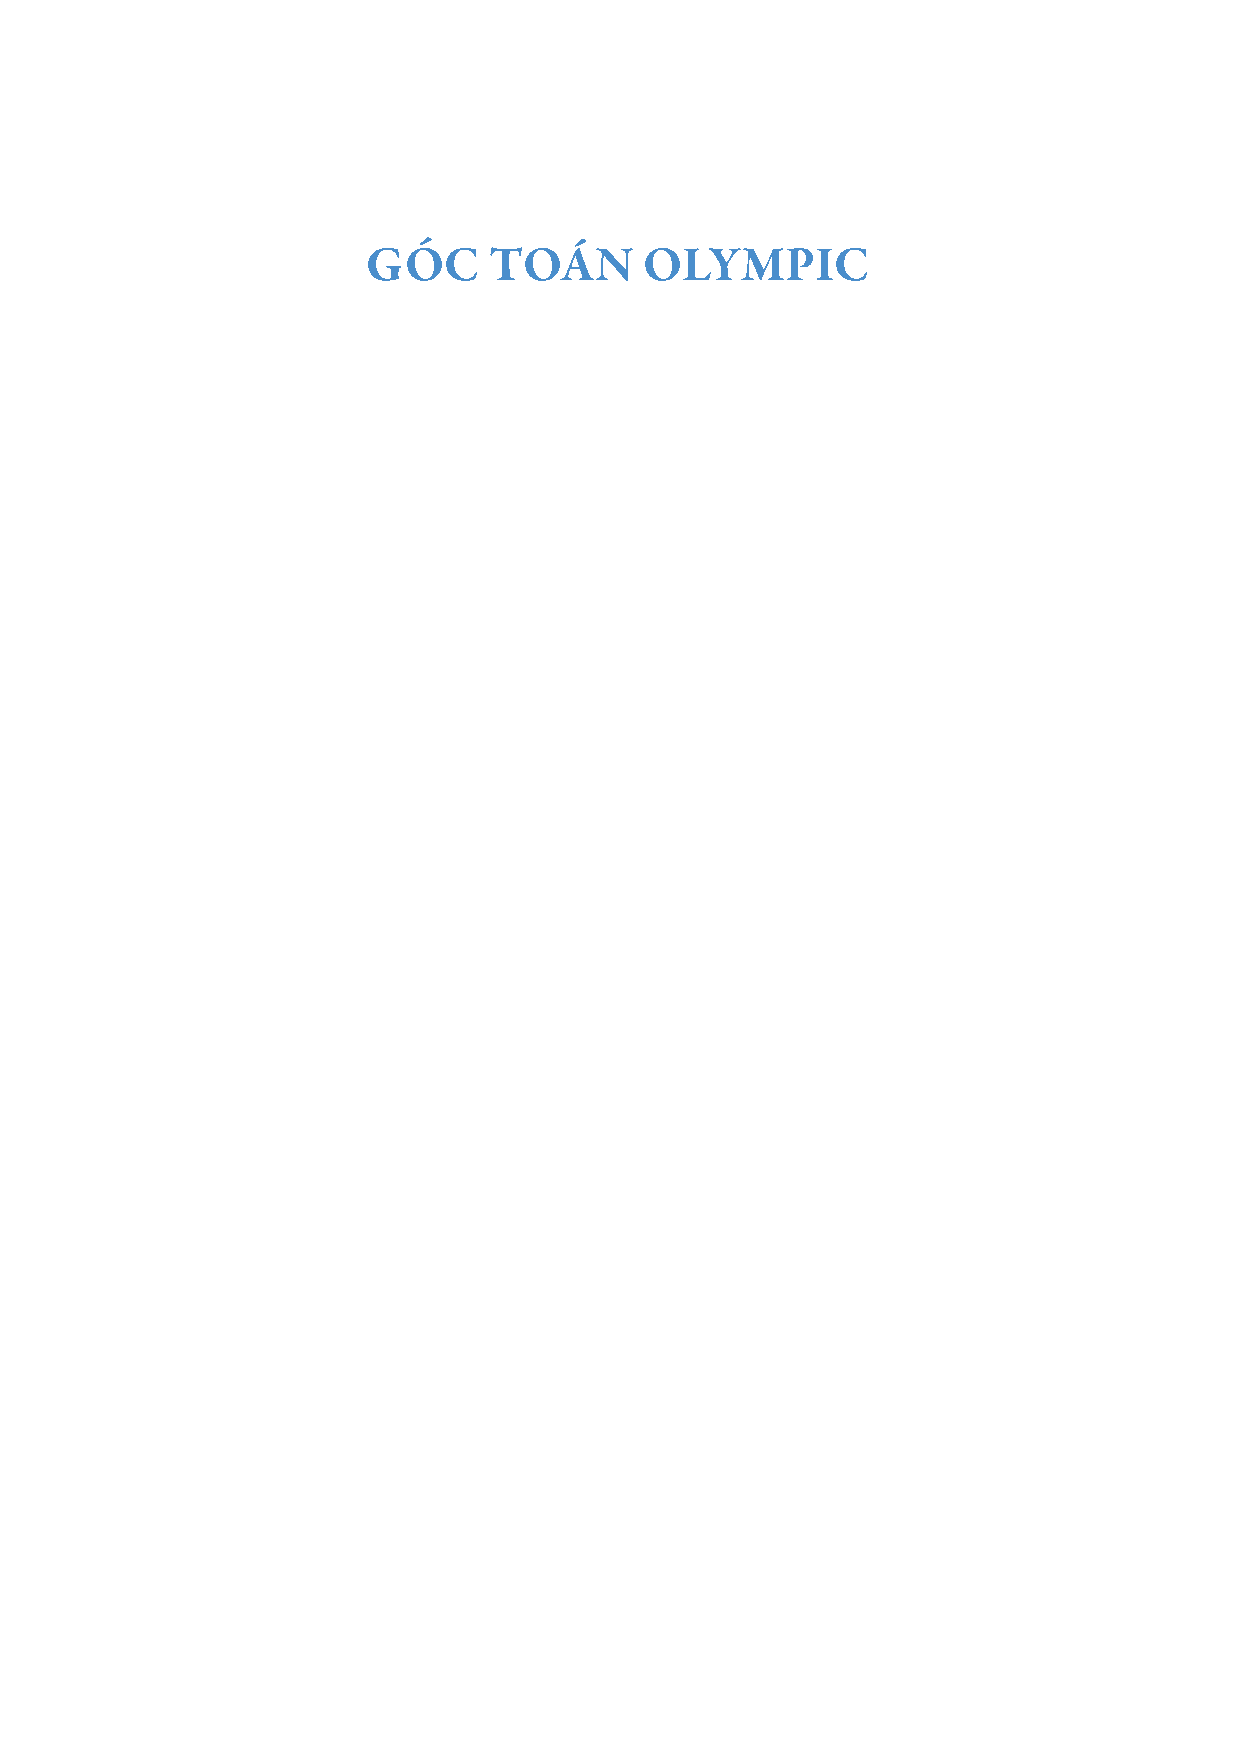
\includegraphics[scale=1]{../tieude1.pdf}}} 
\centering
\endgroup
\vspace*{10pt}

\begin{multicols}{2}
	Trong phần đầu chuyên mục, chúng tôi sẽ trình bày lời giải của các bài toán trong cuộc thi ``Ngày hội Toán học" lần thứ $32$ đăng trong số báo $3/2022$. 
	\begin{figure}[H]
		\vspace*{-5pt}
		\centering
		\captionsetup{labelformat= empty, justification=centering}
		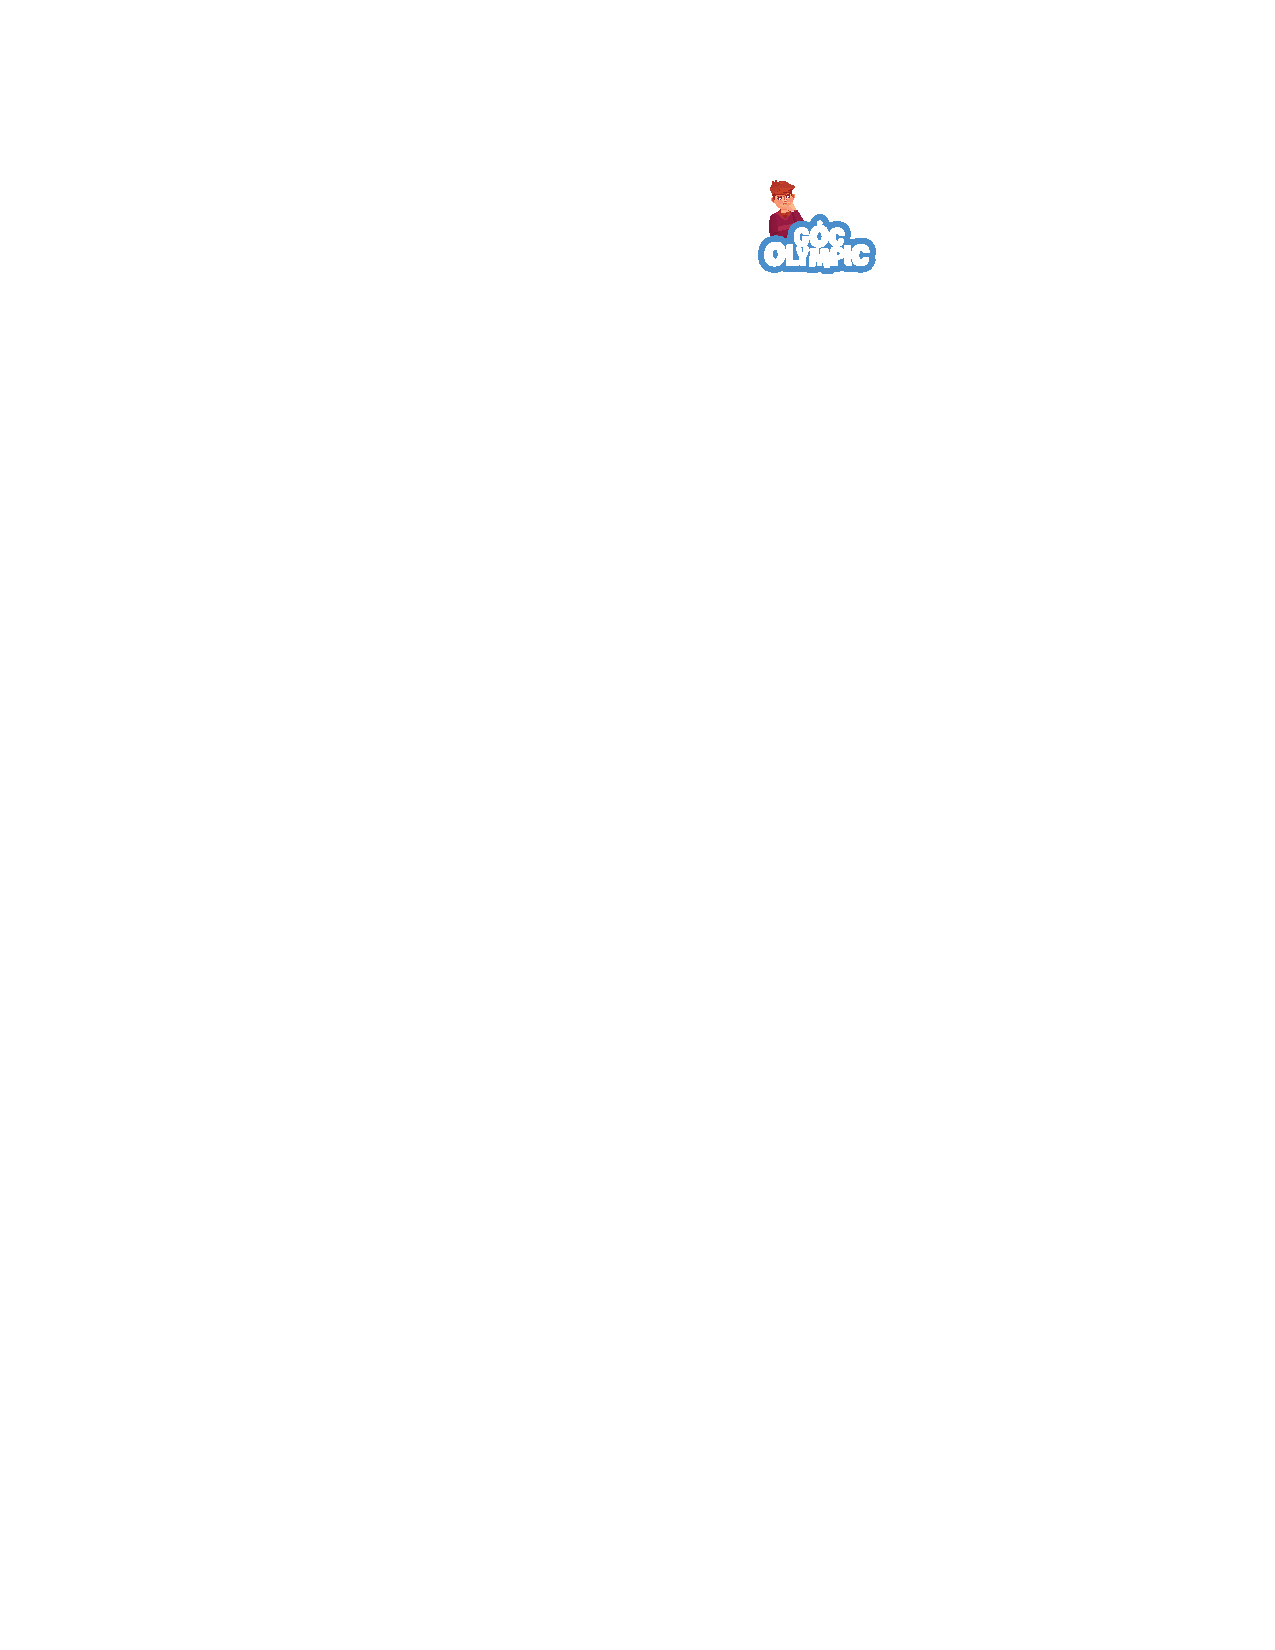
\includegraphics[width= 1\linewidth]{gocolympic}
		\vspace*{-15pt}
	\end{figure}
	{\bf\color{cackithi} OC$\pmb{4.}$} (Lớp $6$) Trong một cửa hàng bán đồ trang sức có bày $15$ viên kim cương. Bên cạnh chúng là các tấm biến chỉ trọng lượng, có ghi $1,2, \cdots,15$ carat. Người bán có một chiếc cân chảo và bốn quả cân nặng $1,2,4$ và $8$ carat. Người mua chỉ được phép cân theo cách như sau: đặt một trong những viên kim cương lên một bên của chiếc cân, các quả cân lên bên kia và kiểm tra xem cân có thăng bằng không. Tuy nhiên, với mỗi lần mượn một quả cân, bạn cần phải trả cho người bán $100$ đồng. Nếu quả cân được lấy ra khỏi cân và không tham gia vào lần cân tiếp theo thì người bán sẽ thu lại nó. Hỏi số tiền ít nhất bạn phải trả để kiểm tra trọng lượng của tất cả các viên kim cương là bao nhiêu?
	\vskip 0.1cm
	{\bf\color{cackithi} Lời giải.} Trước mỗi lần cân, để cân một trọng lượng mới, chúng ta cần mượn thêm hoặc trả lại người bán một hoặc nhiều quả cân. Do đó, chúng ta cần mượn và trả tổng cộng ít nhất $15$ quả cân.
	Đồng thời, sau lần cân cuối cùng, chúng ta còn lại ít nhất một quả cân. Như vậy trong $15$ lần mượn, trả này thì tổng số quả cân mượn nhiều hơn tổng số quả cân trả. Điều này có nghĩa là chúng ta đã mượn ít nhất $8$ quả cân, do đó phải trả cho người bán ít nhất là $800$ đồng.
	\vskip 0.1cm
	Có thể dùng đúng $800$ đồng để kiểm tra trọng lượng của tất cả các viên kim cương như sau:
	\begin{table}[H]
		\vspace*{-5pt}
		\centering
		\resizebox{\columnwidth}{!}{\begin{tabular}{|c|c|l|c|}
				\hline
				\makecell{Khối\\ lượng\\  mượn} & \makecell{Khối\\ lượng\\ trả} & \  Cách cân \    & \makecell{Tổng\\ số\\ tiền}   \\
				\hline
				$1$	&  & $1 \stackrel{?}{=} 1$ & $100$  \\
				\hline
				$2$	&  & $1 + 2  \stackrel{?}{=} 3$  & $200$  \\
				\hline
				& $1$ & $2 \stackrel{?}{=} 2$ & $200$ \\
				\hline
				$4$	&  & $2+4 \stackrel{?}{=} 6$ & $300$  \\
				\hline
				$1$	&  & $1+2+4 \stackrel{?}{=} 7$  & $400$  \\
				\hline
				& $2$ & $1+4 \stackrel{?}{=} 5$ & $400$  \\
				\hline
				& $1$ & $4 \stackrel{?}{=} 4$ & $400$  \\
				\hline
				$8$	&  &  $4+8 \stackrel{?}{=} 12$  & $500$  \\
				\hline
				$1$	&  & $1+4+8 \stackrel{?}{=} 13$ & $600$ \\
				\hline
				$2$	&  & $1+2+4+8 \stackrel{?}{=} 15$ & $700$  \\
				\hline
				& $1$ & $2+4+8 \stackrel{?}{=} 14$ & $700$  \\
				\hline
				& $4$  & $2+8 \stackrel{?}{=} 10$ & $700$  \\
				\hline
				$1$&  &  $1+2+8 \stackrel{?}{=} 11$ & $800$  \\
				\hline
				& $2$ &  $1+8 \stackrel{?}{=} 9$  & $800$  \\
				\hline
				& $1$ & $8 \stackrel{?}{=} 8$  & $800$  \\
				\hline
		\end{tabular}}
		\vspace*{-5pt}
	\end{table}
	Vậy số tiền ít nhất phải trả là $800$ đồng.
	\vskip 0.1cm
	{\bf\color{cackithi} OC$\pmb{5.}$} (Lớp $7$) Cho tam giác đều $ABC.$ Lấy điểm $K$ trên cạnh $AB,$ điểm $L$ và $M$ trên cạnh $BC$ (điểm $L$ nằm trên đoạn $BM$) sao cho
	$KL = KM,BL = 2,AK = 3.$ Tìm độ dài đoạn $CM.$
	\begin{figure}[H]
		\vspace*{-10pt}
		\centering
		\captionsetup{labelformat= empty, justification=centering}
		\definecolor{xdxdff}{rgb}{0.49019607843137253,0.49019607843137253,1}
		\definecolor{uuuuuu}{rgb}{0.26666666666666666,0.26666666666666666,0.26666666666666666}
		\begin{tikzpicture}[line cap=round,line join=round,>=triangle 45,x=1cm,y=1cm,scale=0.8]
			\draw [color= gocco, line width=0.8pt] (0,0)-- (5,0);
			\draw [color= gocco,line width=0.8pt] (5,0)-- (2.5,4.330127018922194);
			\draw [color= gocco,line width=0.8pt] (2.5,4.330127018922194)-- (0,0);
			\draw [color= toanhocdoisong,line width=0.8pt] (1.875334716478179,3.2481750101379796)-- (1,0);
			\draw [line width=0.8pt] (1.5344251501954025,1.5980127233454724) -- (1.3409095662827761,1.650162286792508);
			\draw [color= toanhocdoisong,line width=0.8pt] (1.875334716478179,3.2481750101379796)-- (2.750669432956358,0);
			\draw [color= cackithi,line width=0.8pt] (1.875334716478179,3.2481750101379796)-- (3.750669432956358,0);
			\draw [line width=0.8pt] (2.409759866673582,1.6501622867925085) -- (2.216244282760955,1.5980127233454717);
			\draw [fill=white] (0,0) circle (1.5pt);
			\draw[color=uuuuuu] (-0.1554090558918148,-0.30346876617792) node {$B$};
			\draw [fill=white] (5,0) circle (1.5pt);
			\draw[color=xdxdff] (5.105595104954016,-0.302450506927679956) node {$C$};
			\draw[color=black] (0.52646461936384887,0.25769866723431294) node {$2$};
			\draw[color=black] (2,3.85325166333581533) node {$3$};
			\draw [fill=white] (2.5,4.330127018922194) circle (1.5pt);
			\draw[color=uuuuuu] (2.4667422242757895,4.7692734833990755) node {$A$};
			\draw [fill=white] (1,0) circle (1.5pt);
			\draw[color=xdxdff] (0.9970013793410815,-0.30346876617792) node {$L$};
			\draw [fill=white] (2.750669432956358,0) circle (1.5pt);
			\draw[color=xdxdff] (2.700564631424493,-0.30346876617792) node {$M$};
			\draw [fill=white] (1.875334716478179,3.2481750101379796) circle (1.5pt);
			\draw[color=uuuuuu] (1.6316621987447055,3.583459847144938) node {$K$};
			\draw [fill=white] (3.750669432956358,0) circle (1.5pt);
			\draw[color=xdxdff] (3.700564631424493,-0.30346876617792) node {$T$};
		\end{tikzpicture}
		\vspace*{-5pt}
	\end{figure}
	\textit{Lời giải.} 
	Ta lấy điểm $T$ trên đoạn $MC$ sao cho $MT=2.$ Từ giả thiết $KL=KM$ ta có $\angle BLK= \angle TMK.$ Do đó $\triangle BLK = \triangle TMK $ (c.g.c), suy ra $KB=KT.$ Hơn nữa theo giả thiết $\angle B=60^\circ,$ ta nhận được tam giác $KBT$ đều. Vì vậy $BK=BT,$ do đó $TC=KA=3.$ Ta thu được kết quả $CM= MT + TC=2+3=5.$ 
	\vskip 0.1cm	
	{\bf\color{cackithi} OC$\pmb{6.}$} (Lớp $7$) Năm người bạn đi đến một bờ sông và tìm được một chiếc thuyền có thể chở được cả năm người. Họ quyết định chơi chèo thuyền, mỗi lần một nhóm gồm một hoặc nhiều người sẽ chèo từ bờ này sang bờ bên kia. Liệu các bạn có thể tổ chức chèo thuyền sao cho mọi nhóm người có thể chọn ra từ năm người này đều cùng nhau chèo thuyền qua sông đúng một lần? (Sau khi kết thúc cuộc chơi không nhất thiết phải đưa thuyền và tất cả mọi người quay về bờ nơi xuất phát)
	\vskip 0.1cm
	\textit{Lời giải.} Ta sẽ chứng tỏ bằng phản chứng rằng không thể tổ chức chèo thuyền thỏa mãn điều kiện đầu bài. 
	Thật vậy, giả sử, trái lại, có thể thực hiện được. 
	\vskip 0.1cm
	Có thể chọn ra tổng cộng $2^5-1=31$ nhóm người (khác rỗng)  trong số $5$ người bạn. Như vậy thuyền phải đi qua sông $31$ lần, tức là khi kết thúc cuộc chơi, thuyền sẽ ở bờ sông đối diện.  Giả sử một người $X,$ đi trên chuyến cuối cùng qua sông, khi đó $X$ sẽ phải đi một {\it số lẻ chuyến} vì người này ở bờ đối diện sau khi cuộc chơi kết thúc.
	\vskip 0.1cm
	Mặt khác, số nhóm người chứa $X$ bằng số cách chọn một tập con của tập $4$ người còn lại và bằng $2^4=16.$ Như vậy $X$ phải đi thuyền đúng $16$ lần. Điều này dẫn đến mâu thuẫn. Ta nhận được điều cần chứng minh.  
	\vskip 0.1cm
	Trong phần cuối của chuyên mục kỳ này, chúng tôi sẽ giới thiệu với bạn đọc ba bài toán trong kỳ thi Olympic Toán học của Hà Lan năm học $2020-2021$. Các bài toán này phù hợp với trình độ học sinh khối $6-8$.
	\vskip 0.1cm
	{\bf\color{cackithi} OC$\pmb{13.}$} Bằng cách thay mỗi dấu $\ast$ trong biểu thức 
	\begin{align*}
		1 \ast  2 \ast 3  \ast 4 \ast 5 \ast \cdots \ast 2019 \ast 2020
	\end{align*} bởi dấu $+$ hoặc dấu $-$, ta được một phép tính. Hãy thay các dấu $+$ và $-$ vào như vậy để kết quả của phép tính nhận được là dương và nhỏ nhất có thể.
	\vskip 0.1cm
	{\bf\color{cackithi} OC$\pmb{14.}$} Hình chữ nhật $ABCD$ được chia nhỏ thành bốn hình chữ nhật như trong hình vẽ bên dưới. Diện tích hình chữ nhật $AEIG$ bằng $3$, diện tích hình chữ nhật $EBHI$ bằng $5$ và diện tích hình chữ nhật $IHCF$ bằng $12$. Hỏi diện tích của hình bình hành $AHJF$ bằng bao nhiêu?
	\begin{figure}[H]
		\vspace*{-5pt}
		\centering
		\captionsetup{labelformat= empty, justification=centering}
		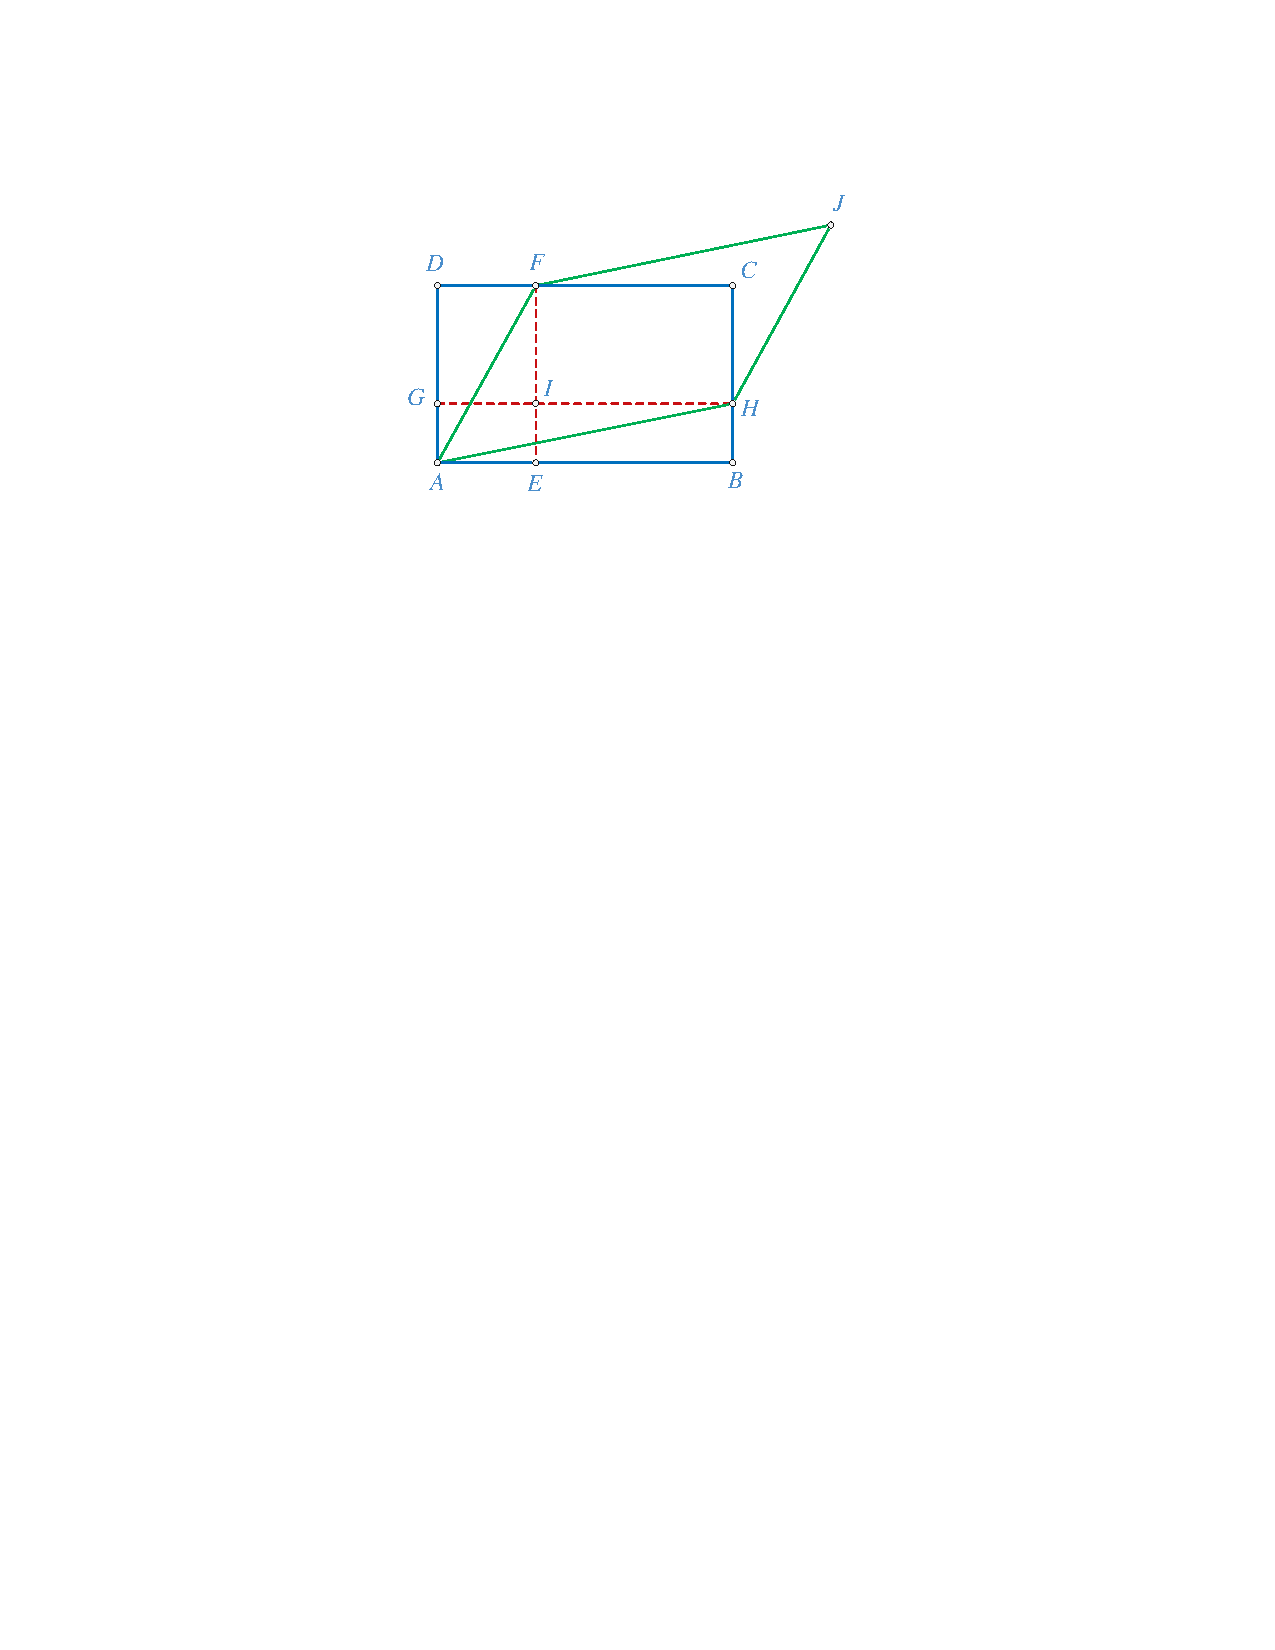
\includegraphics[width= 1\linewidth]{OC14}
		\vspace*{-15pt}
	\end{figure}
	{\bf\color{cackithi} OC$\pmb{15.}$} Chúng ta xét các hàng ngang gồm $2020$ đồng tiền xu, mỗi đồng có mệnh giá $1$, $2$ hoặc $3$. Biết rằng :
	\vskip 0.1cm
	$\bullet$ Giữa hai đồng xu mệnh giá $1$ luôn có ít nhất một đồng xu khác;
	\vskip 0.1cm
	$\bullet$ Giữa hai đồng xu mệnh giá $2$ luôn có ít nhất hai đồng xu khác;
	\vskip 0.1cm
	$\bullet$ Giữa hai đồng xu mệnh giá $3$ luôn có ít nhất ba đồng xu khác.
	\vskip 0.1cm
	Hỏi có bao nhiêu hàng khác nhau gồm $2020$ đồng xu thỏa mãn các điều kiện trên?
\end{multicols}
